\documentclass[hyperref={pdfpagelabels=false}]{beamer}
\usepackage{graphicx,lmodern,subfigure,ulem,color,graphicx,tikz,booktabs}
\usetheme{default}
%\usecolortheme{seahorse}
\definecolor{beamer@blendedblue}{rgb}{0.1,0.5,0.1}
\definecolor{ForestGreen}{RGB}{60, 140, 60}
\setbeamercolor{structure}{fg=beamer@blendedblue}
\setbeamertemplate{navigation symbols}{}
\setbeamertemplate{footline}[frame number]

\usepackage{lmodern}
\newcommand{\spitem}{\vspace{.3cm}\item}

%commands
\newcommand{\elas}{$E_{labor}$}

\title[Capital Structure]{How labor market frictions affect capital structure\\ } 
\author[\insertframenumber/\inserttotalframenumber \hskip 1in 
]{Yasser Boualam, Marco Brianti, Tzuo Hann Law
}
\institute{UNC, BC, BC}

\date{\today}

\begin{document}
\frame{\titlepage \begin{center} Midwest Macro, Pittsburgh, 2017 \end{center} }


\frame{\frametitle{How does labor market frictions affect capital structure?}
\begin{figure}
	\centering
	\begin{itemize}
		\item Modigliani Miller 1958
		\item[] \textbf{Why does capital structure matter at all?}
		\item[] Bankruptcy costs can be high(er) after accounting for stakeholders who might not be (fully) represented at the bargaining table. 
		\item A firm's labor force is one such under-represented entity.
		\item \textbf{This paper:} How does adding capital structure to a workhorse labor market search model affect capital structure decisions?
	\end{itemize}
\end{figure}
}

\frame{\frametitle{What we do}
	\begin{figure}
		\centering
		\begin{itemize}
			\item Highlight empirical findings in the literature that call for the models we present.
			\item Present a simple three period model to highlight the channels.
			\item Present a fully dynamic model and do something...
		\end{itemize}
	\end{figure}
}


\frame{\frametitle{Main channels}
	\begin{figure}
		\centering
		\begin{itemize}
			\item Absent any search frictions, owners of production utilize optimal quantities of debt.
			\item With labor market frictions, the firm partners with a risk averse worker who potentially has the option to quit the partnership.
			\item While this quitting in a partial equilibrium setting benefits workers ex-post, it leads to less entry, less-than-optimal debt use, lower equilibrium wages and ex-ante lower value to workers.
		\end{itemize}
	\end{figure}
}

\frame{\frametitle{Literature}
	\begin{figure}
		\centering
		\begin{itemize}
			\item 
			\item
			\item
		\end{itemize}
	\end{figure}
}

\frame{\frametitle{Empirical observations}
	\begin{figure}
		\centering
		\begin{itemize} 
			\item
			\item
			\item
		\end{itemize}
	\end{figure}
}

\frame{\frametitle{Model without Labor Market Frictions}
	\begin{figure}
		\centering
		\begin{itemize}
			\item Debt is riskless. Borrows pay interest rate $ r $ and return all borrowed capital.
			\item A single agent with initial wealth chooses debt to maximize payoffs in two periods. The output in the first period must be weakly positive.
			\item[] \[\max_D E_2(D) + \phi_e(D)u(b) + (1-\phi_e(D))E_3(D) \] 
			\item where \[E_2(D) = \int_0^1 max(0,\phi(W + D)^\gamma - rD) \hspace{1mm} d\phi\] 
			\[E_3(D) = \int_0^1 max(b,\phi(W + D)^\gamma - rD) \hspace{1mm} d\phi\] 
			\[ \phi_t \in U[0,1] \quad , \quad \phi_e(W + D)^\gamma - rD) = 0 \]
		\end{itemize}
	\end{figure}
}

\frame{\frametitle{Model without Labor Market Frictions: Solution}
	\begin{figure}
		\centering
		\begin{itemize}
			\item The first order condition from earlier yields
			\[\underbrace{\phi_e'}_\text{(+)} \underbrace{(E_3 - u(b))}_\text{(+) , Existence} = E_2' + (1-\phi_e)E_3'\] 
			which shows that the probability of losing the final period output is equated with the marginal gain of more debt.
			\item Financial frictions in the second period reduce the use of debt.
			\item Note here that the owner of the firm can be the worker or the firm in a setting with both agents. 
		\end{itemize}
	\end{figure}
}

\frame{\frametitle{Model without Labor Market Frictions: Solution}
	\begin{figure}
		\centering
		\begin{itemize}
			\item \[E_2' + (1-\phi_e)E_3'\] can further be written as
			\[(2-\phi_e)E_2' + (1-\phi_e)p'(D)\]
			where 
			\[ p'(D) = 2u(b)\frac{d}{dD}\left(\frac{b}{(W+D)^\alpha}\right) + \left[u(b)-u(0)\right]\phi_e' + someshit\] is the marginal effect of debt on the gains from exercising the outside option of home-production in the final period which can be positive or negative.
			\item \[\phi_e' (E_3 - u(b)) -  (1-\phi_e)p'(D) = E_2' + (2-\phi_e)E_2'\] shows us that we get the net effect of financial frictions and technology to use this shit in the 3rd period to balance stuff out.
		\end{itemize}
	\end{figure}
}

\frame{\frametitle{Model without Labor Market Frictions: Comments}
	With limited-liability and a liquidity constraint, a 2 period optimal production problem yields:
	\begin{figure}
		\centering
		\begin{itemize}
			\item Reduced capital utilization relative to the case without liquidity constraint in the second period.
			\item A social safety net (social benebits, $ b $) pushes debt use up because it reduces the cost of bankruptcy in the final period.
		\end{itemize}
	\end{figure}
}

\frame{\frametitle{Labor Market Frictions with Capital Structure}
	Next, we consider how labor market frictions affects debt choice.
	\begin{figure}
		\centering
		\begin{itemize}
			\item Mortensen and Pissarides style search frictions.  
			\item Entrepreneurs/firms own wealth $ W $ and borrow at rate $ r $. Debt is riskless.
			\item Debt choice is made before entry. No new debt or equity.
			\item Wage contracts are specified by \textit{unconstrained wages}, $ \tilde{w} $.
			\item $ \tilde{w} $ is restricted to be identical in both periods.
			\item Perfect commitment assumed. 
			\item No storage technology. 
		\end{itemize}
	\end{figure}
}

\frame{\frametitle{Timing}
	\begin{figure}
		\centering
		\begin{enumerate}
			\item \textbf{Period 0.} Firms with wealth, $ W $ choose debt $ D $ and enter.
			\begin{itemize}
				\item All workers are unemployed.
				\item Firm's post wage contracts, matching occurs.
				\item Unmatched firms exit immediately.
			\end{itemize}
			\item \textbf{Period 1.} Draw productivity $ \phi_1 $.
			\begin{itemize}
				\item If output is weakly negative, match is broken. Firm exits.
				\item Production + consumption occurs.
				\item Unmatched workers consume $ b $.
			\end{itemize}
			\item \textbf{Period 2.} Draw roductivity $ \phi_2 $.
			\begin{itemize}
				\item Separation if output is below $ b $. 
				\item Production + consumption occurs. 
				\item Unmatched workers consume $ b $.
			\end{itemize}
		\end{enumerate}
	\end{figure}
}

\frame{\frametitle{Period production}
	\begin{figure}
		\centering
		\begin{itemize}
			\item Period output is given by
			\item[] \[\phi_t (W + D)^\gamma - Dr\]
			\item If period output is negative, exit occurs.
			\item If output exceeds $ \tilde{w} $, workers are paid $ \tilde{w} $. 
			\item Dividends are positive iff $ (W + D)^\gamma - Dr \ge \tilde{w} $
			\item Don't worry, we have pictures.
		\end{itemize}
	\end{figure}	
}

\frame{\frametitle{Period 1 Wages}
\begin{figure}
	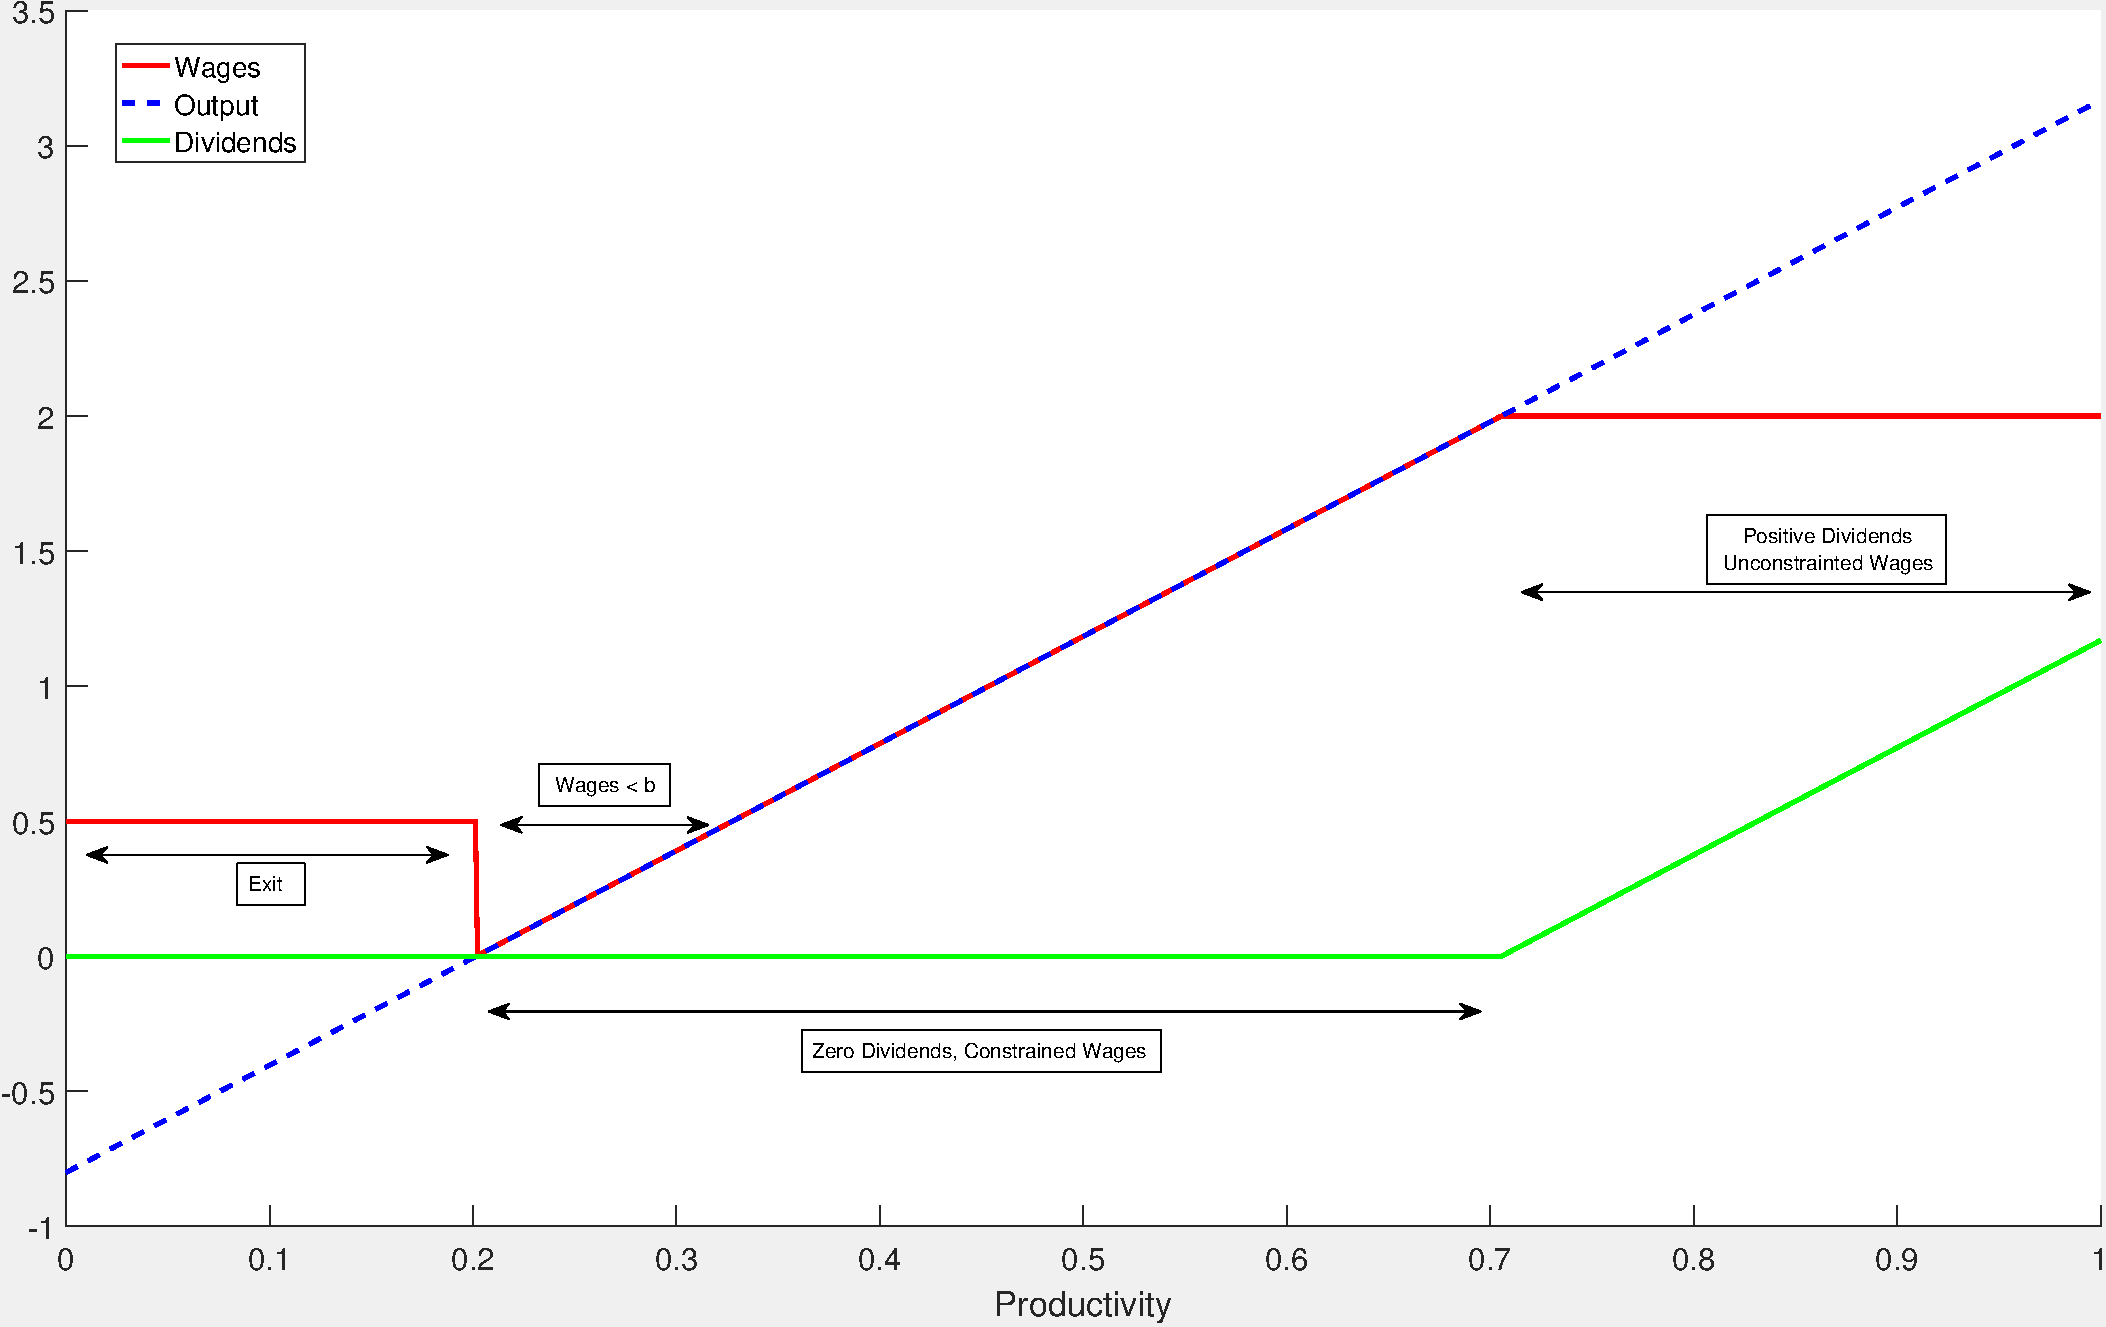
\includegraphics[scale=0.3]{figures/WagePeriod1}
	\label{fig:wageperiod1}
\end{figure}
}

\frame{\frametitle{Period 2 Wages}
	\begin{figure}
		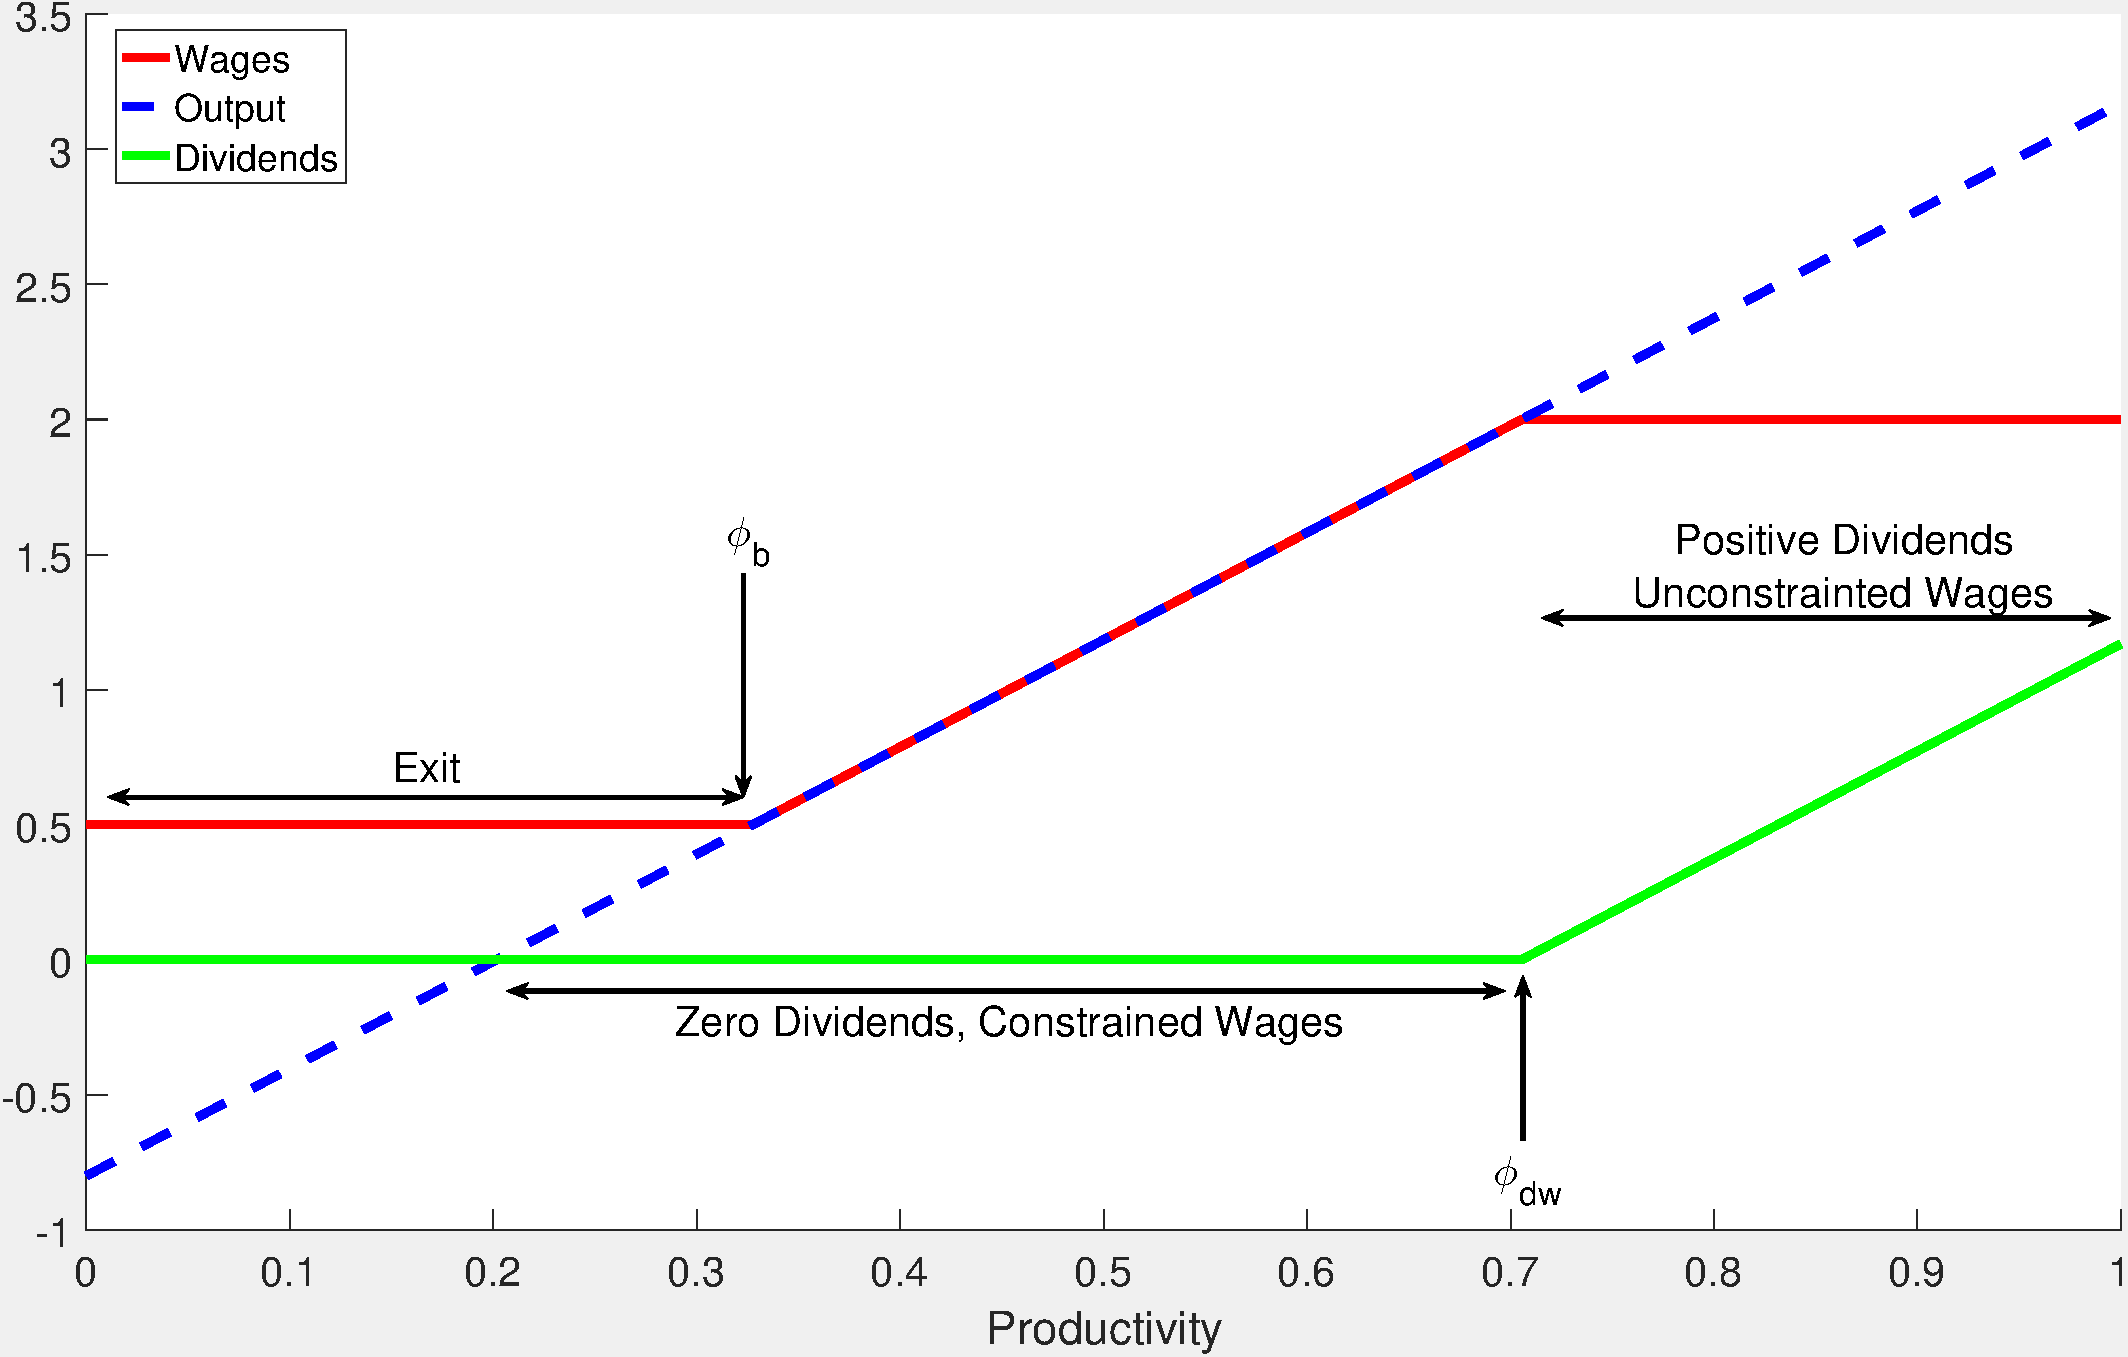
\includegraphics[scale=0.3]{figures/WagePeriod2}
		\label{fig:wageperiod1}
	\end{figure}
}




\frame{\frametitle{Promised Value of a Contract}
	\begin{figure}
	\centering
	\begin{itemize}
		\item $ E(\tilde{w}) $ is the promised value of contract $ \tilde{w} $.
\begin{eqnarray*}
		E(\tilde{w}) &=& \underbrace{\phi_e (1+\beta) u(b)}_\text{$ f(\phi_1) < 0 $, exit} \\
					 &+& \underbrace{\int_{\phi_e}^{\phi_{dw}} f(\phi_t) d\phi}_\text{wage = output, zero div.} + \underbrace{\int_{\phi_{dw}}^1\tilde{w}d\phi}_\text{wage = $ \tilde{w} $, positive div.} \\
					 &+& (1-\phi_e)\underbrace{\left( \phi_b u(b) + \int_{\phi_b}^{\phi_{dw}} f(\phi_t) d\phi + \int_{\phi_{dw}}^1\tilde{w}d\phi\right)}_\text{final period wages} 
		\end{eqnarray*}
		\item[] where $ \phi_e $, $ \phi_b $ and $ \phi_dw $ are the cutoffs seen earlier.
	\end{itemize}
\end{figure}	
}

\frame{\frametitle{Worker's Problem}
	\begin{figure}
		\centering
		\begin{itemize}
		\item $ \theta(\tilde{w}) $ is market tightness for a given contract
		\item $ p(\theta(\tilde{w})) = m(\theta(\tilde{w}))/s $ is job finding probability
		\item \[U = \max_{\tilde{w}} \underbrace{p(\theta(\tilde{w})) E(\tilde{w})}_\text{indifference condition} \]
	\end{itemize}
\end{figure}	
}

\frame{\frametitle{Expected Profits of a Contract}
	\begin{figure}
		\centering
		\begin{itemize}
			\item $ V(\tilde{w}) $ is the value of contract $ \tilde{w} $ taking debt as given
			\begin{eqnarray*}
				V(\tilde{w}) &=& \underbrace{\phi_e (1+\beta) \cdot 0}_\text{$ f(\phi_1) < 0 $, exit} \\
				&+& \underbrace{\int_{\phi_e}^{\phi_{dw}} 0 \hspace{1mm} d\phi}_\text{wage = output, zero div.} + \underbrace{\int_{\phi_{dw}}^1f(\phi_1)-\tilde{w} \hspace{1mm}d\phi}_\text{wage = $ \tilde{w} $, positive div.} \\
				&+& (1-\phi_e)\underbrace{\left( \phi_b \cdot 0 + \int_{\phi_b}^{\phi_{dw}} 0 \hspace{1mm} d\phi + \int_{\phi_{dw}}^1f(\phi_2)-\tilde{w} \hspace{1mm}d\phi\right)}_\text{final period wages} 
			\end{eqnarray*}
			\item[] where $ \phi_e $, $ \phi_b $ and $ \phi_dw $ are the cutoffs seen earlier.
		\end{itemize}
	\end{figure}	
}

\frame{\frametitle{Firms's Problem}
	\begin{figure}
		\centering
		\begin{itemize}
			\item $ q(\theta(\tilde{w})) = m(\theta(\tilde{w}))/v $ is vacancy filling probability
			\item[] \[W = \max_{\tilde{w};D} \underbrace{q(\theta(\tilde{w})) V(\tilde{w};D)}_\text{indifference condition} \]
			\item Optimal debt choice will involve firms choosing debt and posting the corresponding profit maximizing contract $ \tilde{w} $ which maximizes ex-ante value, $ U $ for workers. 
		\end{itemize}
	\end{figure}	
}


\frame{\frametitle{Results: Wages}
	\begin{figure}
		\centering
		\begin{itemize}
			\item
		\end{itemize}
	\end{figure}	
}

\frame{\frametitle{Results: Entry}
	\begin{figure}
		\centering
		\begin{itemize}
			\item
		\end{itemize}
	\end{figure}	
}

\frame{\frametitle{Results: Ex-ante Value of Unemployment}
	\begin{figure}
		\centering
		\begin{itemize}
			\item
		\end{itemize}
	\end{figure}	
}

\frame{\frametitle{Results: Profits condition on Matching}
	\begin{figure}
		\centering
		\begin{itemize}
			\item
		\end{itemize}
	\end{figure}	
}

\frame{\frametitle{Dynamic Model with Labor Market Frictions}
	\begin{figure}
		\centering
		\begin{itemize}
			\item 
			\item
			\item
			\item
			\item
		\end{itemize}
	\end{figure}
}

\frame{\frametitle{Conclusion}
	\begin{figure}
		\centering
		\begin{itemize}
			\item 
			\item
			\item
			\item
			\item
		\end{itemize}
	\end{figure}
}

\end{document}
